
\NeedsTeXFormat{LaTeX2e}
\documentclass[11pt]{article}


\usepackage{setspace}
\usepackage{amsmath}
\usepackage{amssymb}
\usepackage{epsfig}
\usepackage{fancybox}
\usepackage{listings}
\usepackage{url}
\usepackage{pgfgantt}
\usepackage{tikz}
\usepackage{siunitx}
\usepackage{graphicx}
\usepackage{float}

\setlength{\textheight}{9.5in}
\setlength{\textwidth}{6in}
\setlength{\oddsidemargin}{.25in}
\setlength{\topmargin}{-0.7in}  % changed from -.25 by RSR on 1/21/07
%\parindent .5in    % commented out by RSR 1/21/07

%put words in the hyphenation statement if you want to enforce
%how LaTeX should break them (or not) at the end of a line.
%\hyphenation{repre-sen-tations problems exact linear}
\hyphenation{itself}
\usepackage{cite}

\makeatletter
\ganttset{
    prog default/.initial=100,
    prog/.code={
        \pgfutil@in@{:}{#1}
        \ifpgfutil@in@
            \pgfqkeysalso{/pgfgantt}{@prog={#1}}
        \else
            \pgfqkeysalso{/pgfgantt}{@prog={\pgfkeysvalueof{/pgfgantt/prog default}:#1}}
        \fi
    },
    @prog/.code args={#1:#2}{
        \pgfqkeysalso{/pgfgantt}{progress=100, progress label text={\hspace{0.02cm}#2}}
    }
}
\makeatother
\ganttset{progress label anchor/.append style={text=red}}

\title{\vspace{-1.7cm}Final Report for the Hacking Challenge Creation
\\[0.3in]
\bfseries Predictable Session IDs \& Steganography
\\[0.1in]
}
\author{Alexander Daniel Nikolaos Lelidis, Andr\'{e} Baptista \'{A}guas, \\ Ard Kastrati, Khalid Aldughayem, Uro\v{s} Te\v{s}i\'{c}}

\begin{document}

\maketitle

\begin{abstract}
This challenge combines two different tasks from Web Security and Steganography. It addresses the problem of the predictable sessions and the security through obscurity. The idea of this challenge is to first bypass the authorization in the HTTP level by hijacking a session with a predictable session ID. Secondly, the attacker must extract the secret information which is hidden by using steganography instead of cryptography. 
\end{abstract}


\section{Requirements}

\begin{itemize}
\item A program to reverse the Mersenne Twister MT-19937. A program that solves this can be found in \url{https://github.com/eboda/mersenne-twister-recover}.
\item A program needed for requesting the 624 session IDs and storing them in a file so that the Mersenne Twister can recover the pseudorandom generator. A simple program that does this is given in the following:
\begin{verbatim}
import requests

with open("mersenneCookies.txt","w") as output:

  for i in range(625):
  
    r = requests.post('http://<ip address>:5000/login', data = 
                      {'user':'user1', 'password':'password1'})
    output.write(str(r.cookies['netsecLoginCookie']) + "\n")
    requests.post('http://<ip address>:5000/logout',cookies=r.cookies)
\end{verbatim}
where \texttt{<ip address>} must be set to the IP address of server. 
\item A cookie editor in your web browser. We recommend you use developer tools in Firefox (\textit{Tools} $\rightarrow$ \textit{Web Developer} $\rightarrow$ \textit{Toggle Tools}).
\item Basic knowledge about steganography.
\end{itemize}

\section{Learning goals}
There are three different learning goals in this challenge:
\begin{enumerate}
\item \textit{If the attacker can control the pseudorandom generator, then he can control everything.} \\
	As discussed in the lecture, controlling the pseudorandom generators is the perfect attack, since it is almost impossible to detect. Generating not truly random numbers are very hard to detect. 
	
\item \textit{The security of an algorithm should rely solely on the secrecy of the key} \cite{katzlindell} \\
Never use an algorithm, the security of which relies solely on the fact that the algorithm is secret. One speaks of security through obscurity. The advantage of steganography over cryptography alone is that the intended secret message does not attract attention to itself as an object of scrutiny. However, \textit{once} it is known that something secret is being hidden, steganography is insecure from today’s point of view. With security through obscurity it is not possible to establish standard algorithms, which can be tested from others. As a countermeasure, Kerckhoffs's principles have been established. 
In 1833, Auguste Kerkhoffs stated six design principles for military ciphers in \cite{Kerckhoffs83} and one of them is \cite{katzlindell}:
\begin{itemize}
\item The cipher method should not be required to be secret, and it must be able to fall into the hands of the enemy without inconvenience.
\end{itemize}
In the scenario that is given in this project, \textit{Alice} misapplied the purpose of steganography. \textit{Alice's} goal is to keep her data confidential, in case someone manages to log into her account. However, in case someone attacks \textit{Alice}, then \textit{Alice} \textit{is already a suspect} and hence the attacker can assume that secret data can be hidden by using steganography. Once this happens, the purpose of using steganography is pointless. It is worth mentioning that the Kerkhoff's principle has been often ignored, which led to fatal results. 
	\item \textit{Adding more different unsecure mechanisms in the system doesn't make it more secure, since the attacker can simply bypass all of them one after another.}\\
	
\end{enumerate}


\section{Mission}
Alice and Bob need to share secrets with each other. However, they don't trust the security of the chat in the social network they are using. One day Alice reads about the \textit{steganography} and she was amazed. As a beginner in modern cryptography, she thought that this has to be the best way to share secrets. Without further thinking she arranges a meeting with Bob and they decide to hide their data in different pictures that they send to each other. On the one hand, the website is known to love the Mersenne Twister\footnote{The Mersenne Twister (MT 19937) is used as PRNG in many programming languages. However, given at least 624 outputs of a Mersenne Twister we can restore its internal state and find all other consecutive numbers.} whenever a random generator is needed and on the other hand Alice must log in every 5 minutes to this website. Alice was right about one thing: \textit{The website is indeed not secure and there is a way to bypass the login page}. Ironically, the \textit{steganography} is not much more secure than that. The agency for national security of the United States ``ANS'' suspects that \textit{Alice} is preparing to commit a crime. As a secret agent, an account has been already opened for you in the social network. The credentials are the following:
\begin{itemize}
	\item username: \texttt{user1}
	\item password: \texttt{password1}
\end{itemize}
Your mission, should you choose to accept it, is to bypass the login page for \textit{Alice}, read the data exchanged between them and extract the secret message that they exchanged with each other.

\section{Mitigation}
\begin{enumerate}
\item Use cryptographically secure pseudorandom number generator (CSPRNG).
\item Use standard encryption schemes from modern cryptography (instead of steganography) for confidentiality (such as AES, RSA, El-Gammal etc).
\end{enumerate}


\section{Type of Challenge}
Online

\section{Category}
Web Security \& Cryptography

\section{Hints}
\begin{itemize}
\item Mersenne Twister is used to generate the session keys!
\item Consider the channels (red, green and blue) of the image \textit{separately} and look if you can find information in some of the bits of every channel. 
\end{itemize}

\section{Setup}
\begin{itemize}
\item Start the client and the server using VirtualBox\footnote{Make sure that the machine is connected with Host-only adapter. See README file if any problems occur.} or VMWare. The credentials are:
\begin{itemize}
	\item Client
	\begin{verbatim}
		password: 123
	\end{verbatim}
	\item Server
		\begin{verbatim}
			username: user
			password: ERenaRboRy
		\end{verbatim}
\end{itemize}
\item Find the IP address of the server by running \texttt{ifconfig} on the server inside the server machine.
\item Open the browser and enter the following URL: \texttt{<ip address of the server>:5000}
\end{itemize}


\section{Solution}

\subsection{Idea of the solution}
After logging in, we see a harmless profile with chat and news. However, if we look at the cookies, we will see a \texttt{netsecLoginCookie}. If we log out and log in again, we see that the value changed. Multiple logins tell us that the cookie is always less than 32-bits, and its value changes randomly. That randomness is the key. Mersenne twister is not a cryptographically secure pseudorandom generator. There are two possible attacks on this PRNG:
\begin{itemize}
\item We can download Untwister (\url{https://github.com/altf4/untwister}) presented at BSides in Las Vegas in 2014. We only need a few generated values to obtain the seed. Unfortunately, this is done by brute force. It is possible to do it this way because seed has 32-bits, but it still takes 3-4 hours in the general case. We decided to use a small seed value, so this attack takes only a few seconds.
\item  If we look at the implementation of the Mersenne twister, we can see that it is just a big XOR machine with 624 numbers as its state. Every number is transformed (tempered), and output as a random value, until all 624 numbers are used. The state is then transformed together, and the cycle continues. Tempering can be inverted, and we can easily reconstruct the entire state of the PRNG, and guess every subsequent number. This requires 625 consequent integers (state plus one more number in case of refresh). For this attack to work, only we are allowed to log in when we poll the server. In case that the \textit{Alice} logs in, we must start again.
\end{itemize}
After we obtain the next state, we should replace the cookie in our browser with the next generated value, and wait for \textit{Alice} to log in again. Once we gain access to the \textit{Alice's} account, we can see that she is up to no good. By inspecting the chat, we obtain an image that shows the next target. The image looks like a city, but isn't identifiable. This is likely a steganography challenge. The data is hidden in the LSB (Least Significant Bit) of every channel (red, green and blue) separately.

\subsection{Step-by-step instructions}

\begin{itemize}
\item Generate 625 session IDs by using python3 with the given program in the requirement section.
 
\item Get the state of the generator of the Mersenne Twister and predict some of the next session IDs, by using the Mersenne twister recoverer from \url{https://github.com/eboda/mersenne-twister-recover}. We recommend you to generate the next 50 session IDs in advance. The programs that generates the first 625 session IDs and the next 50 ones can be found in the client machine under the following folder: \texttt{Documents/attack}.

\item Every 5 minutes \textit{Alice} will log into the website, so you may have to wait for \textit{Alice} to log in for the first time. After 5 minutes, you can either try to change the cookie to the next one, or you can log out and log in again to see what is the current session ID in order to avoid any mistakes. After you log in for the second time, you will know that the previous session ID is the session ID of the \textit{Alice}.  
 
\item Change your session ID to \textit{Alice's} session ID (Session hijacking). In order to edit the session ID, you must:
\begin{itemize}
	\item Open developer tools (\textit{Tools} $\rightarrow$ \textit{Web Developer} $\rightarrow$ \textit{Toggle Tools})
	\begin{figure}[H]
    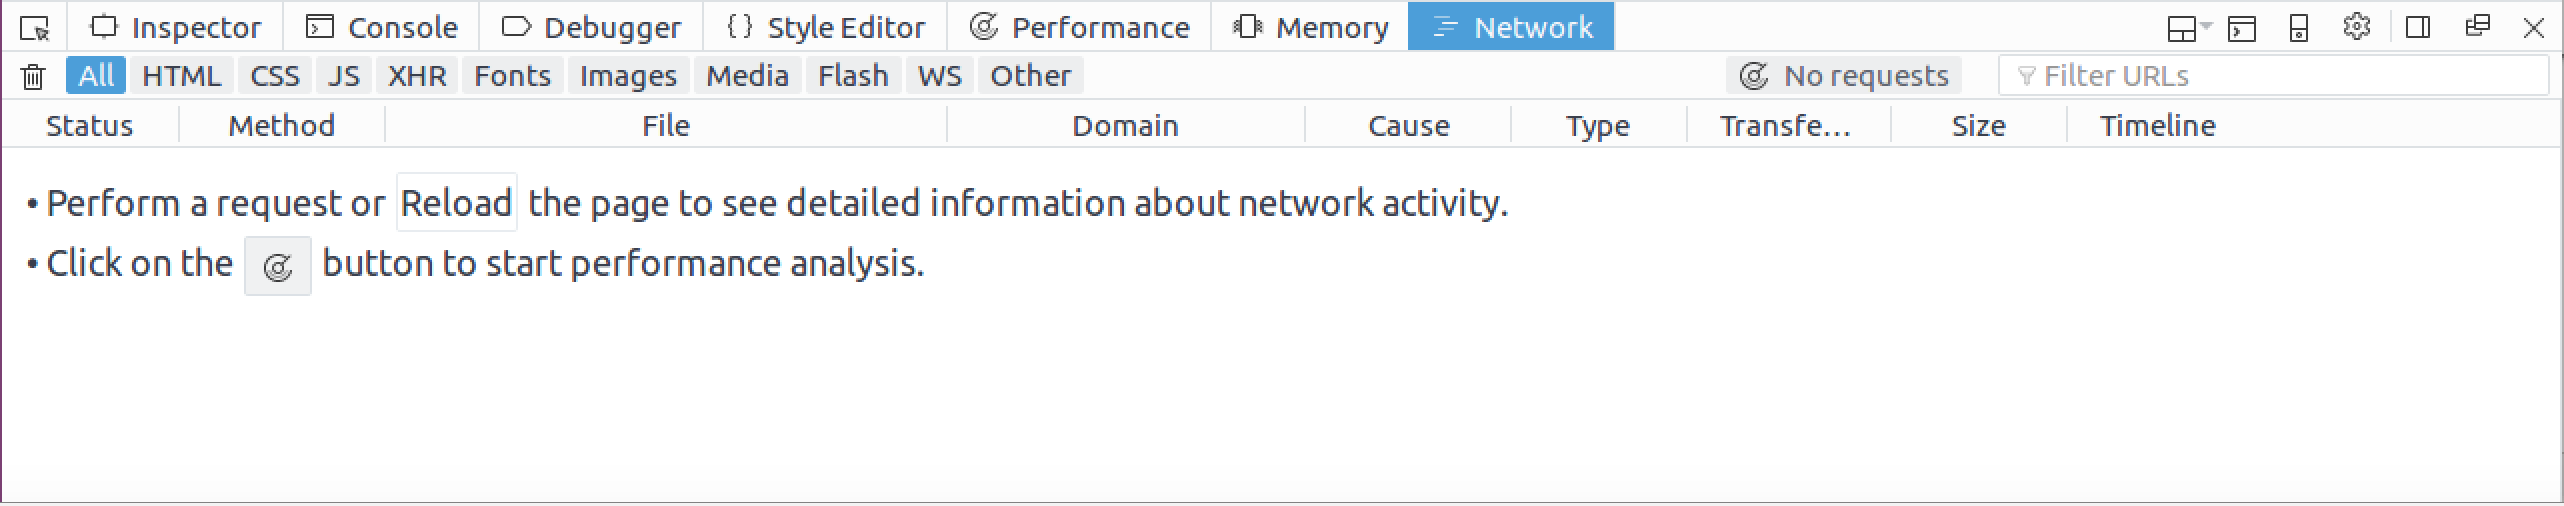
\includegraphics[width=\linewidth]{images/developerTools.png}
	\end{figure}
	\item Enable the storage inspector via the settings of the developer tools
	\begin{figure}[H]
    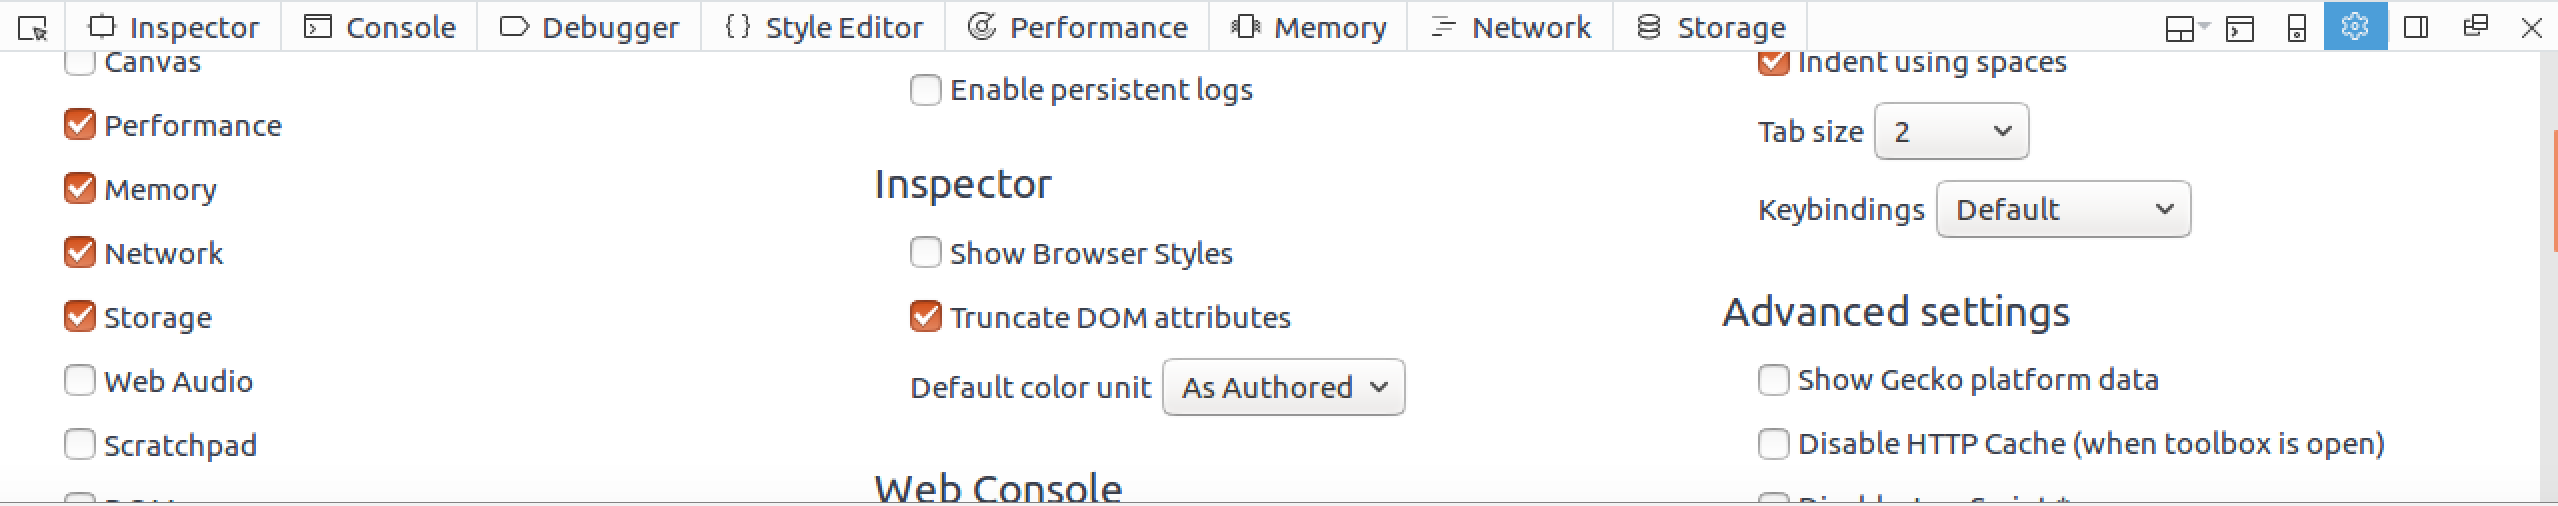
\includegraphics[width=\linewidth]{images/storageEnable.png}
	\end{figure}
	\item Change the \texttt{netsecLoginCookie} to the \textit{Alice's} session ID.
	\begin{figure}[H]
    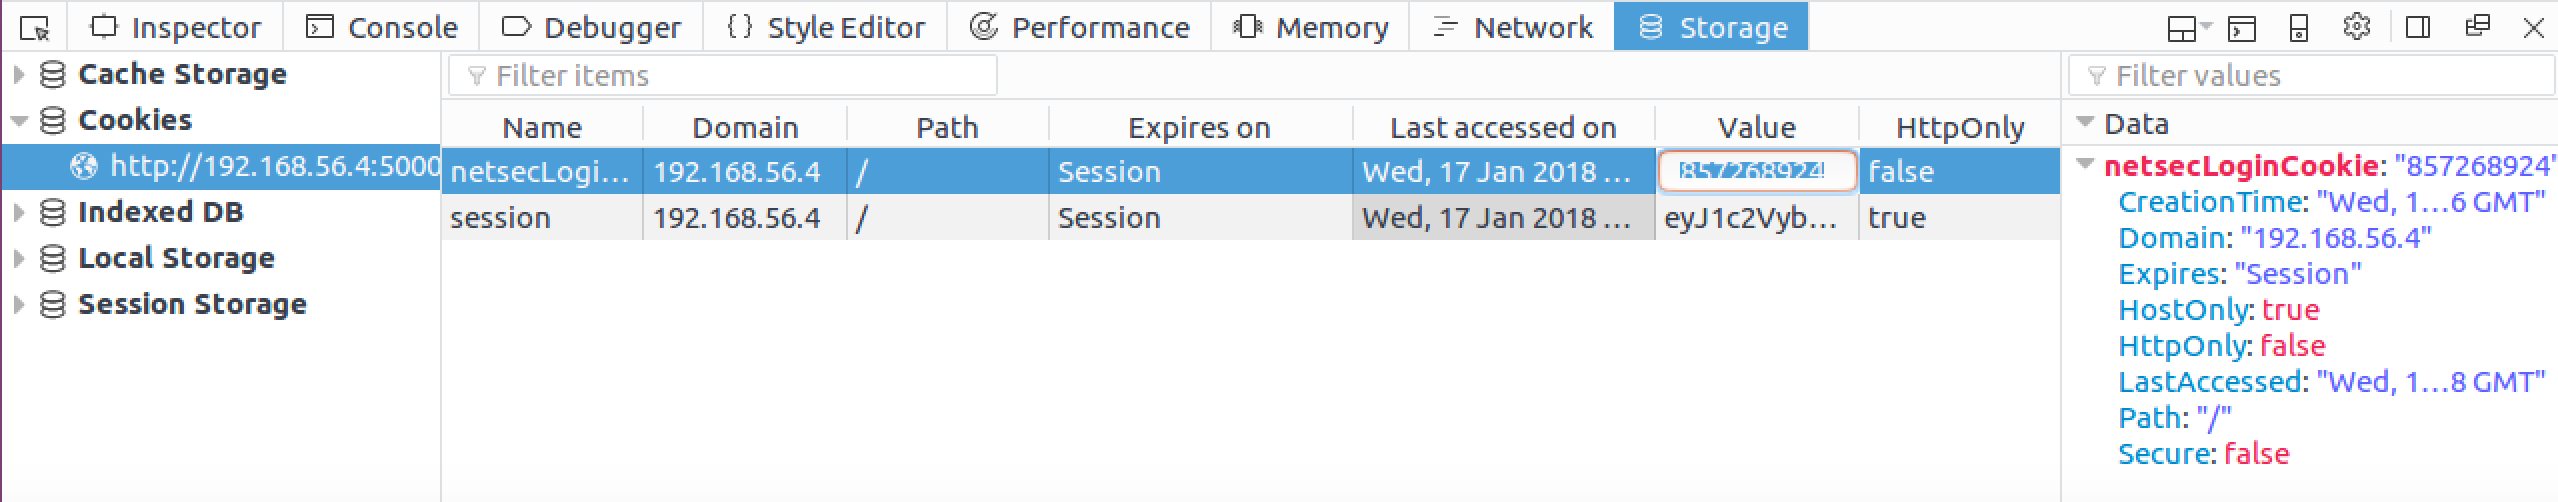
\includegraphics[width=\linewidth]{images/changeCookie.png}
	\end{figure}
	\item Open \texttt{http://<ip address>:5000}.
	\begin{figure}[H]
    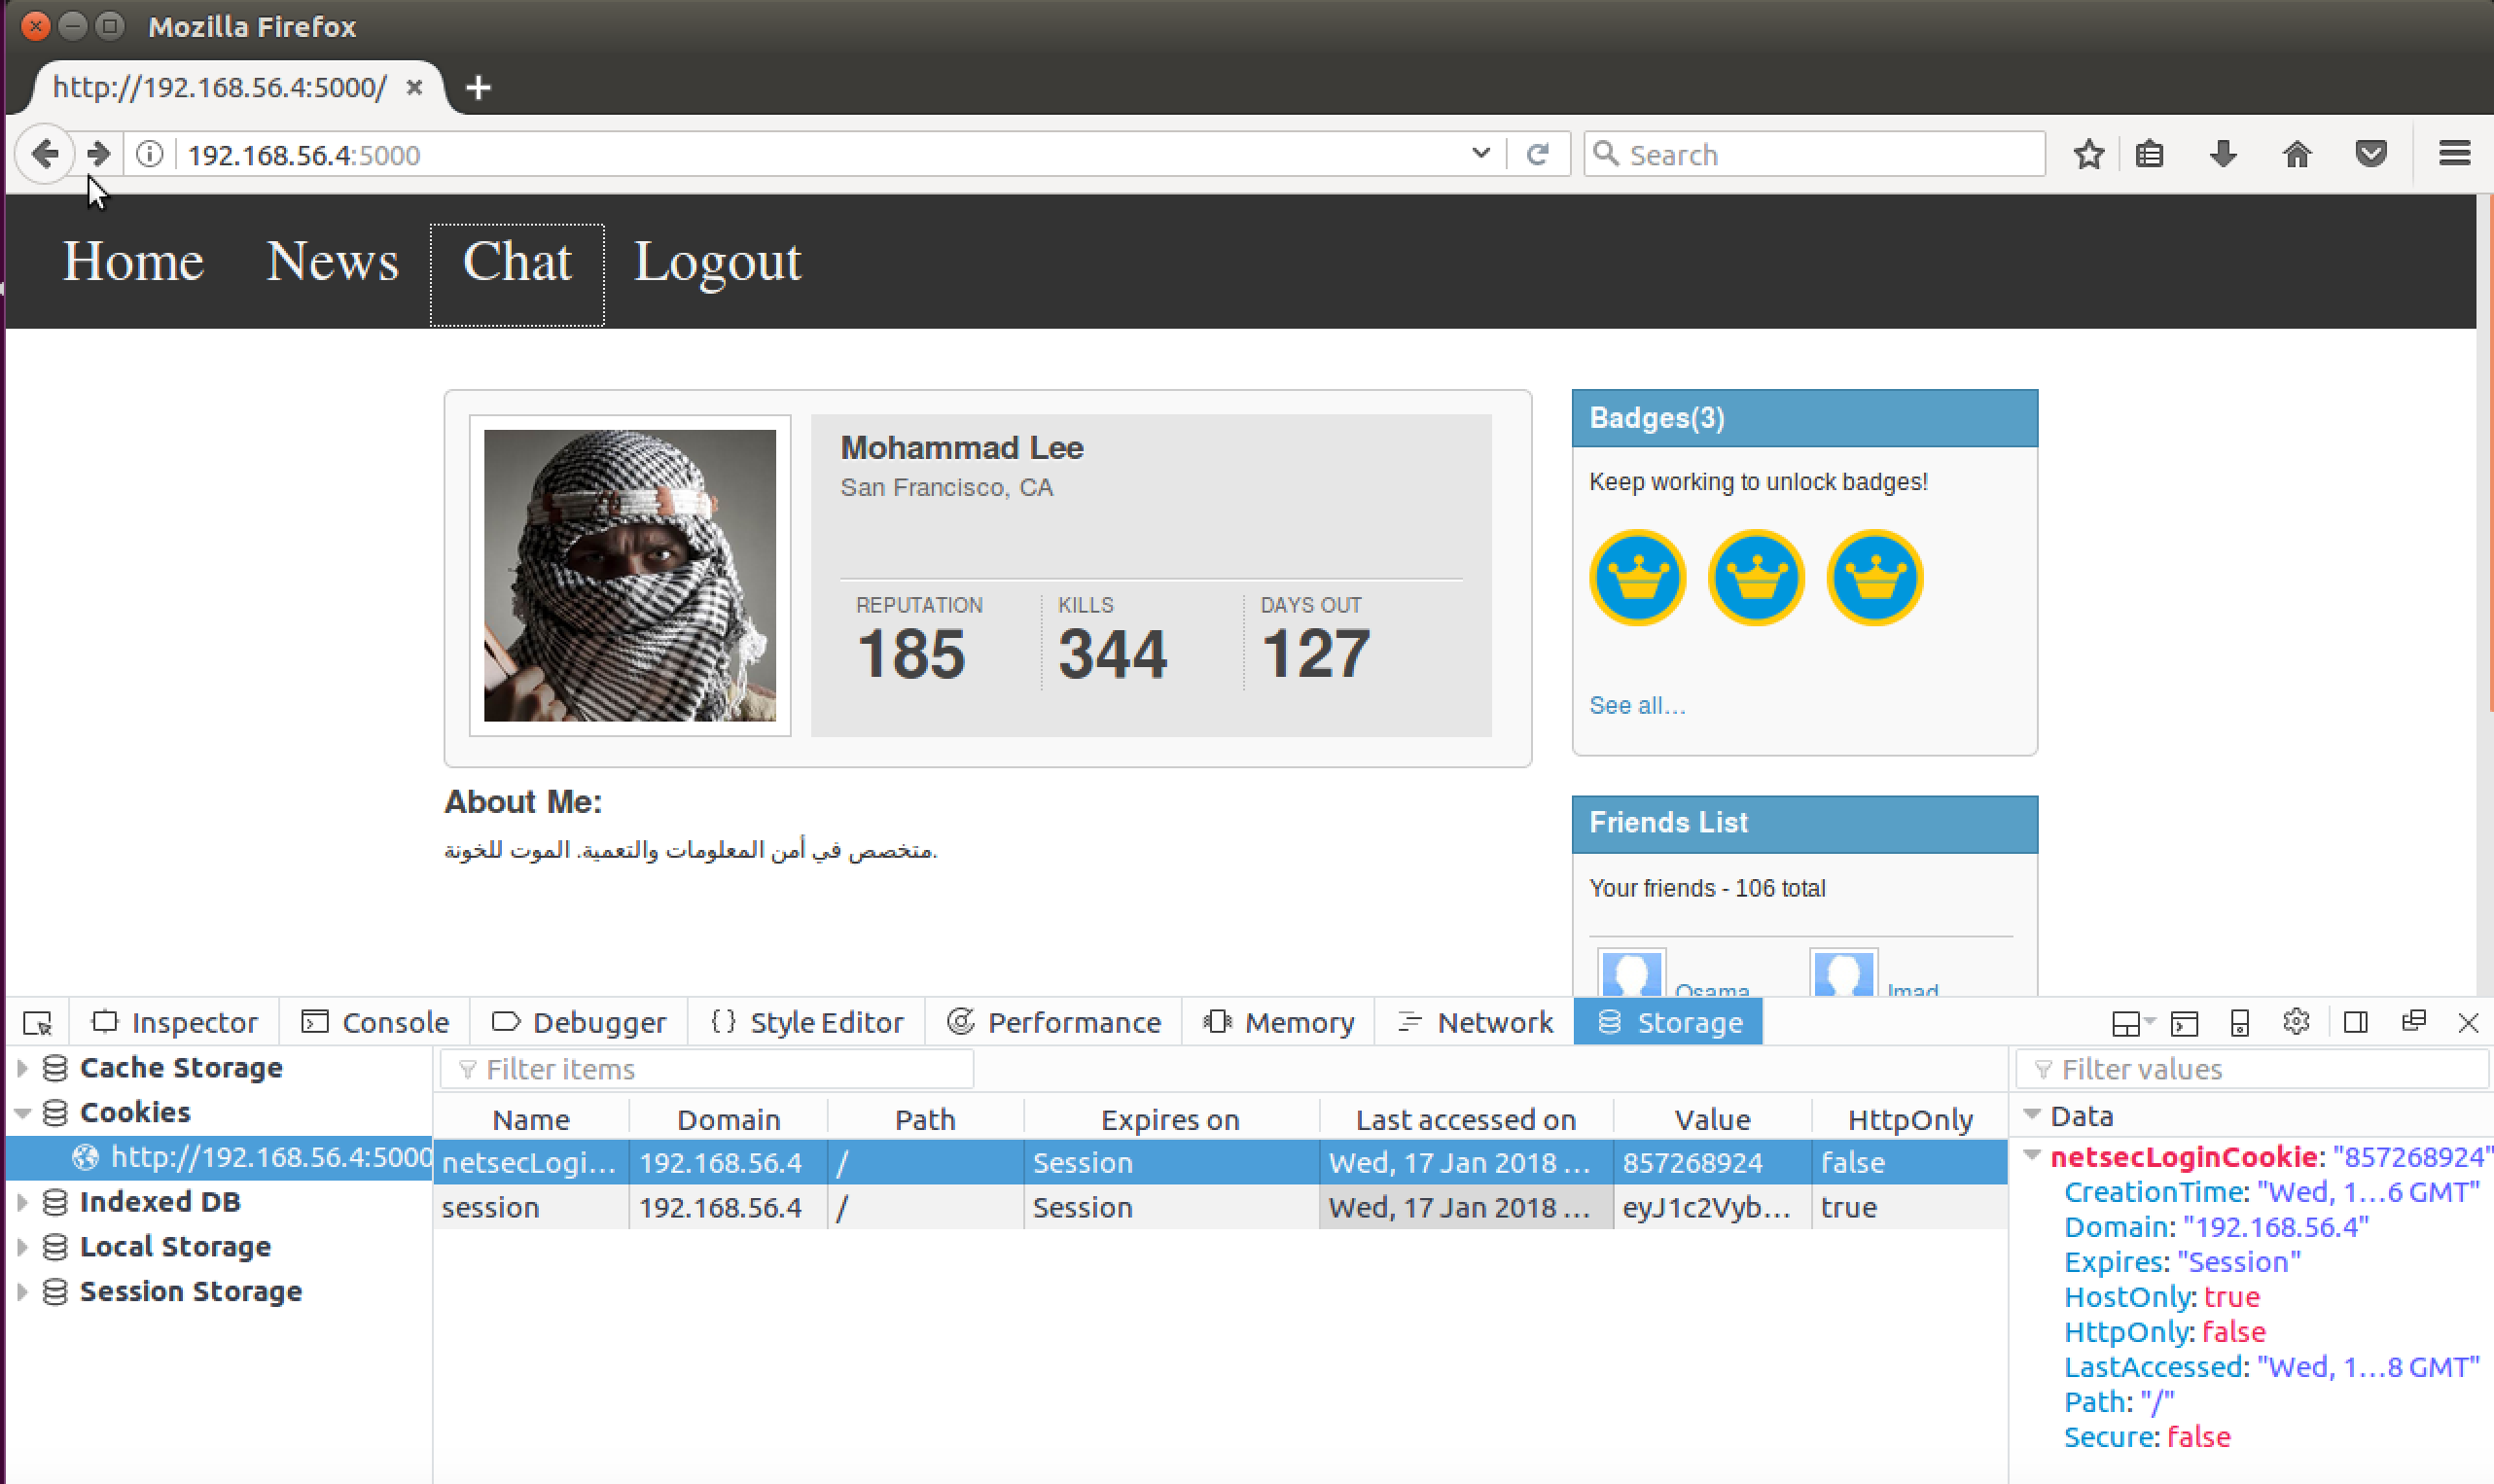
\includegraphics[width=\linewidth]{images/adminPage.png}
	\end{figure}
\end{itemize}

\item Go to the chat and download the image that was sent to you.
\begin{figure}[H]
    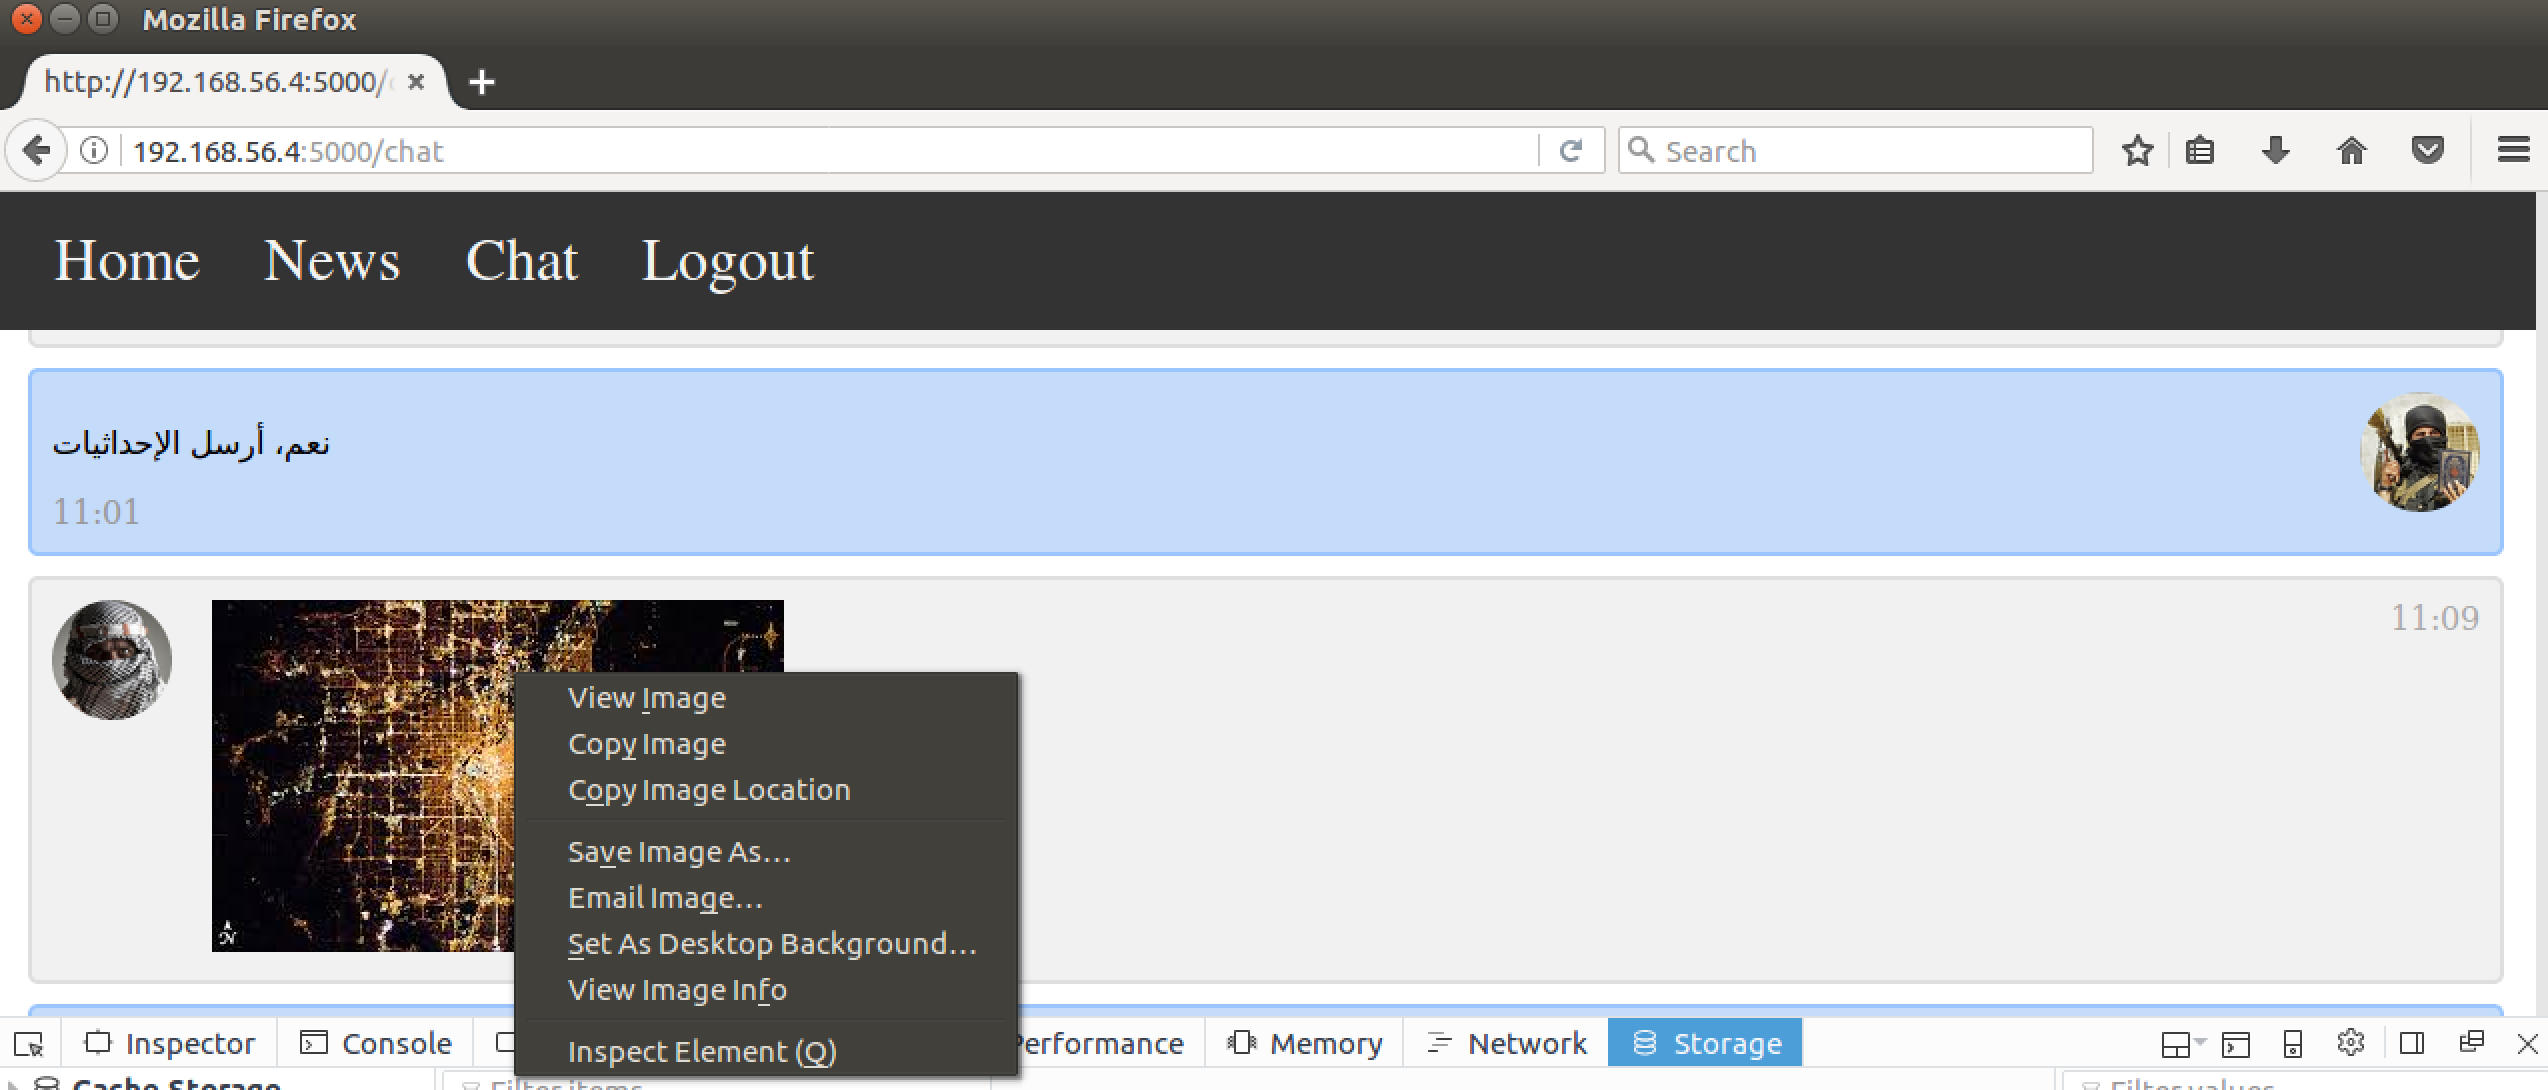
\includegraphics[width=\linewidth]{images/steganography.png}
	\end{figure}
\item Extract the secret data by separating all three different channels (red, green, blue) from the image and get the LSB in every channel. You can do this by using the following program:

\begin{verbatim}
import png
import sys

filename = sys.argv[1]

imageReader = png.Reader(filename)

image = imageReader.asRGBA()

width = image[0]
height = image[1]
pixels = list(image[2])

binaryRed = ""
binaryGreen = ""
binaryBlue = ""


counter = 0

for i in range(height):

    row = pixels[i]

    for j in range(width):
        binaryRed += str(row[4*j]%2)
        binaryGreen += str(row[4*j+1]%2)
        binaryBlue += str(row[4*j+2]%2)

        counter += 1

binaryRed = [binaryRed[i:i+8] for i in range(0, len(binaryRed), 8)]
binaryGreen = [binaryGreen[i:i+8] for i in range(0, len(binaryGreen), 8)]
binaryBlue = [binaryBlue[i:i+8] for i in range(0, len(binaryBlue), 8)]

redText = "".join([chr(int(x,2)) for x in binaryRed])
greenText = "".join([chr(int(x,2)) for x in binaryGreen])
blueText = "".join([chr(int(x,2)) for x in binaryBlue])

print(redText)
print(greenText)
print(blueText)
\end{verbatim}
\item If we take the least significant bit of every color in the image, the start of the red channel will form a string \ang{38;53;52} N \ang{77;02;11} W. These are the coordinates of the White House. Other two channels have Easter eggs in them. Hurry up and protect the president!
\end{itemize}

\section{Implementation}

The implementation of the system can be divided into two parts:
\begin{itemize}
	\item \textit{Creating a website with a chat in it and with predictable session IDs.} \\
	 The website is very simple. The website is written in Python and Flask framework. Only few features are supported in the website. 
\begin{itemize}
\item Log In\\
The web server provides an interface where the clients can log in via the internet by using his/her credentials. 
					
\item Home\\
Information about the account can be found. This data is frozen and no further functions are provided.
				
\item News\\
Latest news in the world. This data is also frozen and no further functions are provided, since they are not relevant for the challenge.
				
\item Chat\\
Since a feature that provides a chat isn't really necessary, we created just a static chat, where the users can supposedly communicate. This means that the chat is frozen and contains some static text which can only be read.
				
\end{itemize}			 
	 
	  Next implementation step, was to generate session IDs by using the Mersenne Twister. This was also very simple since the twister MT-19937 is already provided in Python as a default pseudorandom generator, which has a period length of $2^{19937}$. We use always the same seed $1337$ in the beginning. For simplicity during the implementation of the website, we chose all communication between the web server and the client to be sent by using HTTP --- the data is \textbf{not} encrypted and \textbf{not} authenticated. This means, other active attacks are also possible (e.g. Man in the Middle). They are however not part of this challenge. 

	  
	\item \textit{Generating an image where some information is hidden by using steganography.}\\
	We created a script, which hides the data in a picture. The created picture was then added inside the static chat afterwards.
\end{itemize}

The implementation can be found in the web server under the folder \texttt{netsec-project}.
\begin{spacing}{1}
  \bibliographystyle{plain}
  \bibliography{mybibtexDB}
\end{spacing}

\end{document}
